\documentclass[a4paper,12pt]{book}
\usepackage[utf8]{inputenc}
\title{}
\author{Rachel Morris}
\date{\today}

\usepackage{rachwidgets}
\usepackage{fancyhdr}
\usepackage{lastpage}
\usepackage{dirtree}
\usepackage{boxedminipage}

\newcommand{\laChapter}{2.2\ }
\newcommand{\laClass}{CS 210\ }
\newcommand{\laSemester}{Fall 2017\ }
\newcounter{question}

\pagestyle{fancy}
\fancyhf{}
\lhead{CS 210}
\chead{Fall 2017}
\rhead{Ch \laChapter Exercise}
\rfoot{\thepage\ of \pageref{LastPage}}
\lfoot{\scriptsize By Rachel Morris, last updated \today}

\renewcommand{\headrulewidth}{2pt}
\renewcommand{\footrulewidth}{1pt}

\begin{document}

    %\toggletrue{answerkey}
    \togglefalse{answerkey}

    %------------------------------------------------------------------%
    %- Exercise Begin -------------------------------------------------%
    %------------------------------------------------------------------%

    %------------------------------------------------------------------%
    \section*{1. More definitions}

        \begin{intro}{Modulus}
            ``In computing, the modulo operation finds the remainder after
            division of one number by another (sometimes called modulus).

            Given two positive numbers, a (the dividend) and n (the divisor),
            a modulo n (abbreviated as a mod n) is the remainder of the Euclidean division of a by n."
            \footnote{From https://en.wikipedia.org/wiki/Modulo\_operation}

            \begin{center}
                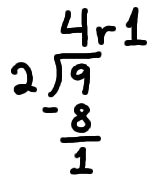
\includegraphics[height=3cm]{images/ch2-1-division.png}

                $9$ mod $2 = 1$
            \end{center}

            If we're dividing $a$ by $b$, the result is a quotient $q$.
            If we're calculating $a$ mod $b$, the result is the remainder $r$.

            \begin{center}
                We can also write this out as: \\
                $ a = b \cdot q + r $,
                where $0 \leq r < b$, and $q$ and $r$ are the only two integers
                that will satisfy the equation.
            \end{center}
        \end{intro}

        \begin{intro}{Rational numbers}
            In mathematics, a rational number is any number that can be
            expressed as the quotient or fraction p/q of two integers,
            a numerator p and a non-zero denominator q.[1] Since q may be equal to 1,
            every integer is a rational number.
            \footnote{From https://en.wikipedia.org/wiki/Rational\_number}

            The set of rational numbers is written as $\mathbb{Q}$.
        \end{intro}

        \newpage
        % - QUESTION --------------------------------------------------%
        \stepcounter{question}
        \begin{questionNOGRADE}{\thequestion}
            Solve the following modulus problems.

            \paragraph{Example:} Solve 13 mod 5 \\
                \begin{answer} 13 / 5 = 2, \tab 13 mod 5 = 3, \tab $13 = 5 \cdot 2 + 3$ \end{answer}

            \begin{enumerate}
                \item[a.] 9 mod 7
                    \iftoggle{answerkey}{ \begin{answer}
                    9 mod 7 = 2; \tab $9 = 7 \cdot 1 + 2$
                    \end{answer} }{ { ~\\ \raisebox{0pt}[0.5cm][0pt]{  } } }

                \item[b.] 5 mod 2
                    \iftoggle{answerkey}{ \begin{answer}
                    5 mod 2 = 1; \tab $5 = 2 \cdot 2 + 1$
                    \end{answer} }{ { ~\\ \raisebox{0pt}[0.5cm][0pt]{  } } }

                \item[c.] 15 mod 3
                    \iftoggle{answerkey}{ \begin{answer}
                    15 mod 3 = 0; \tab $15 = 3 \cdot 5 + 0$
                    \end{answer} }{ { ~\\ \raisebox{0pt}[0.5cm][0pt]{  } } }

                \item[d.] -7 mod 2
                    \iftoggle{answerkey}{ \begin{answer}
                    -7 mod 2 = 1; \tab $-7 = 2 \cdot -4 + 1$
                    \end{answer} }{ { ~\\ \raisebox{0pt}[0.5cm][0pt]{  } } }

            \end{enumerate}
        \end{questionNOGRADE}

        \hrulefill

        % - QUESTION --------------------------------------------------%
        \stepcounter{question}
        \begin{questionNOGRADE}{\thequestion}
            Prove the following propositions:

            \begin{enumerate}
                \item[a.] If $a$ divides $b$ and $a$ divides $c$, then $a$ divides $b + c$.
                    \footnote{From Discrete Mathematics by Ensley and Crawley}

                    \begin{hint}{\ }
                        Start with: $b = ak$ and $c = aj$ and calculate $b+c$.
                    \end{hint}

                    \iftoggle{answerkey}{ \begin{answer}
                        $b = ak, c = aj \tab => b + c = ak + aj \tab => a(k+j) $
                    \end{answer} }
                    { { ~\\ \raisebox{0pt}[1cm][0pt]{  } } }

                \item[b.] If $a$ divides $b$ and $c$ divides $d$, then $ac$ divides $bd$.
                    \footnote{From Discrete Mathematics by Ensley and Crawley}

                    \begin{hint}{\ }
                        Start with: $b = ak, d = cj$ and calculate $bd$.
                    \end{hint}

                    \iftoggle{answerkey}{ \begin{answer}
                    $b = ak, d = cj \tab => bd = (ak)(cj) \tab => (ac)(kj) $
                    \end{answer} }
                    {  }

            \end{enumerate}
        \end{questionNOGRADE}


\end{document}
